

When performing software tasks in large and complex software systems, software developers typically consult several different kinds of artifacts that assist them in their work~\cite{Starke2009, Meyer2017}. For example, 
when incorporating a new API library needed for a new feature, a developer might consult official API documents and guidelines~\cite{robillard2011field, umarji2008archetypal} or she might consult question-and-answer forums for functionality, security and performance-related topics~\cite{parnin2012, silva2019}.



Much critical information in this and other non-source code types of artifacts 
contain data in the form of unstructured text~\cite{Bavota2016} and 
a developer must read the text to find the information that is \textit{relevant} to the task being performed.
However, the sheer amount of information \textit{within} these natural language artifacts may prevent a developer from comprehensively assessing what is useful to their task~\cite{Murphy2005}. Just within one kind of document, API
documentation, studies have shown that it can take 15 minutes or more
of a developer's highly constrained time to identify 
information needed to perform a particular software task~\cite{endrikat2014, Meyer2017}
and a developer that fails to locate all, or most, of the information needed
 will have an incomplete or incorrect basis from which to perform a software task~\cite{Murphy2005}.





\section{Scenario}
\label{cp1:example}




To illustrate challenges in locating information useful for a task, let us consider an open-source mail client\footnote{\url{https://github.com/k9mail/k-9}}.
Figure~\ref{fig:android-notifications-task} shows a task---in the form of a GitHub issue---that indicates that the app notifications 
are not working as expected\footnote{\url{https://github.com/k9mail/k-9/issues/1741}}. 


A developer assigned to this issue might require additional knowledge to understand and resolve the bug~\cite{ko2007, Li2013, sillito2006}. 
More than often, this knowledge can be acquired from a developer's peers~\cite{singer2011}. 
However, the fragmented and distributed nature of software development  
may prevent the developer from accessing their peers~\cite{ko2007},
what often makes  them seek online web resources for information 
that may assist in completing the task-at-hand~\cite{Xia2017, rao2020}.
For example, the developer might refer to changelogs 
about the latest Android version or perhaps
consult community forums to find if any other developers had a similar issue~\cite{parnin2012}. 


% \medskip


% \newpage


Finding information in API documents and other web resources can be a time-consuming
and cognitively frustrating process~\cite{Begel2008,
robillard2011field}. 
As Figure~\ref{fig:android-search-results} shows, querying `\textit{android notification quick actions}'
reveals that there are 28,000,000 potential pages related to this topic
and even if the developer restricts their search to the results shown in the figure, reading all of their content would take approximately 30 minutes or more\footnote{using a standard reading metric of 200 words per minute~\cite{Just1980}} of a developer's highly constrained time~\cite{endrikat2014, Meyer2017}. 


\begin{figure}
    \centering
    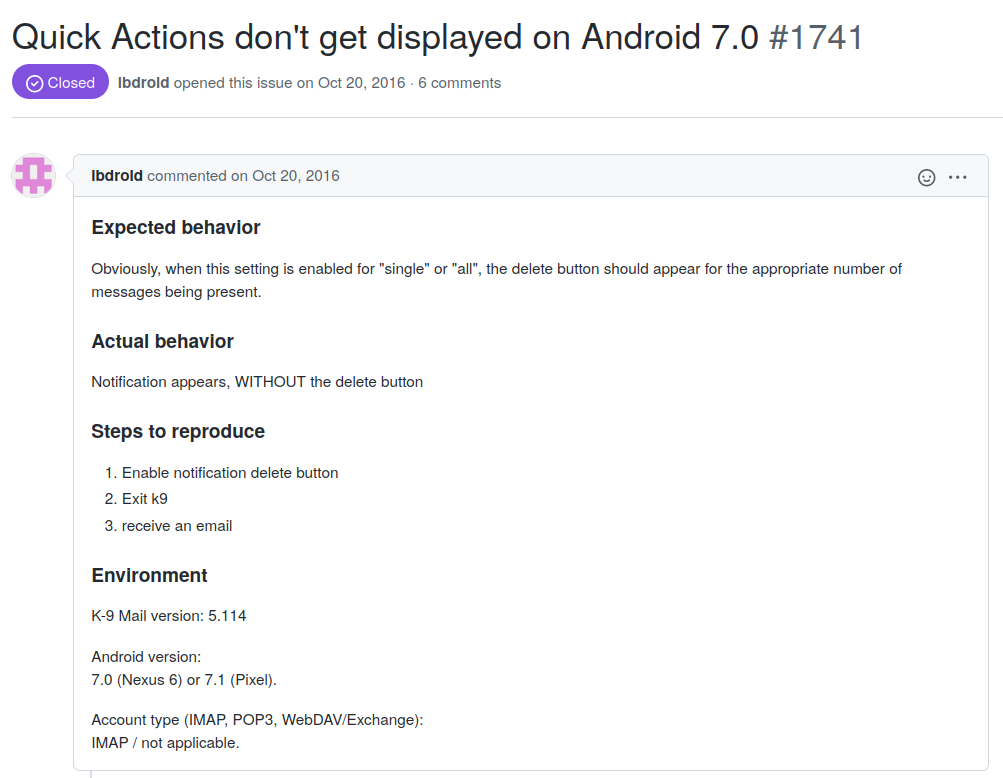
\includegraphics[width=.75\textwidth]{cp1/android-quick-actions}
    \caption{k-9 mail GitHub issue \#1741 indicating that quick actions don't get displayed on Android 7.0}
    \label{fig:android-notifications-task}
\end{figure}



It is also worth noting that not all of the content of these artifacts is relevant to the developer's task. 
For instance, Figure~\ref{fig:android-notifications-api-page} shows a snapshot 
of the Android notifications documentation, where among  
the many topics presented on the page (right-hand side), only the `\textit{notification actions}' portion (under focus) might be relevant to this developer's task. 
When reading this document, or any of the other documents of potential relevance to a task, a developer 
faces the burden of having to sift through large amounts of
irrelevant text (e.g., because of legacy information, boilerplate text, or because it is intended for another audience) to filter just those parts that are relevant to them~\cite{Robillard2015}. 


% \newpage

As tasks become more complex~\cite{Pirolli2007, Bystrom1995}, a developer often has to combine multiple pieces of text (from the same artifact or different ones) to understand what is needed for the task-at-hand~\cite{Piorkowski2016}. For example, Figure~\ref{fig:android-notifications-api-page} shows that details about adding
action buttons is explained further in a different web page.
If no tool support is provided, much of the process of locating relevant text in the 
artifacts relevant to a task fall on the developer's shoulders~\cite{gonccalves2011, Ko2006a, Bystrom1995}.



\vspace{3mm}
\begin{figure}
\centering    
\parbox{\textwidth}{% 
\centering
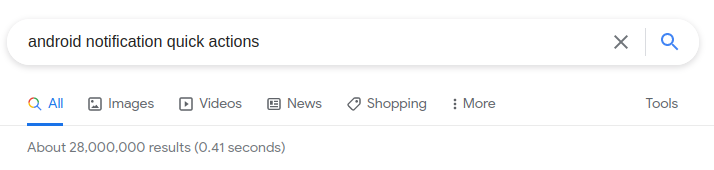
\includegraphics[width=.80\textwidth]{cp1/task-google-search}
}
\parbox{\textwidth}{%
\centering
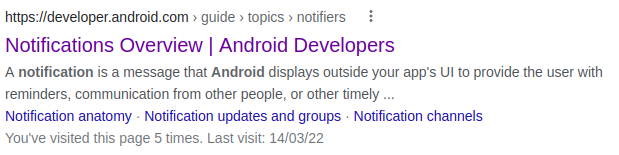
\includegraphics[width=.70\textwidth]{cp1/api-documentation-search-result}
}
\parbox{\textwidth}{%
\centering
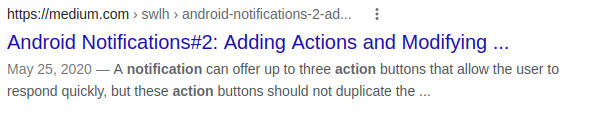
\includegraphics[width=.70\textwidth]{cp1/misc-documentation-search-result}
}
\parbox{\textwidth}{%
\centering
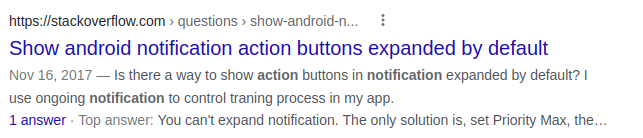
\includegraphics[width=.70\textwidth]{cp1/so-documentation-search-result}
}
\parbox{\textwidth}{%
\centering
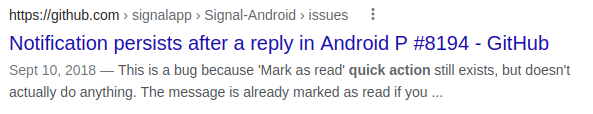
\includegraphics[width=.70\textwidth]{cp1/git-documentation-search-result}
}
\caption{Search results showing artifacts of potential interest to the Android quick notifications issue}
\label{fig:android-search-results}
\end{figure}





Researchers have long recognized the value of assisting developers in 
identifying information of relevance within the natural language
text of a software artifact. 
Often these approaches use a combination of \acf{NLP} and \acf{ML} techniques to identify potentially useful textual fragments. 
For example, some \acs{NLP} techniques rely on regular expressions describing a sequence of tokens
representing words or linguistic elements for the automatic identification 
of relevant text~\cite{Bavota2016, Chaparro2017}. 
Other \acs{ML}-based techniques use extractive text summarization 
to produce a summary of an artifact's content
and a developer might use this summary to find key information
that may help them complete their task~\cite{Bavota2016}.



When \acs{NLP} or \acs{ML} techniques are applied to software engineering artifacts, researchers often 
consider pre-defined kinds of tasks.
For example, the discourse patterns used by {\small DeMIBuD}~\cite{Chaparro2017} 
assist bug triage tasks. However, the text detailing a bug's observed or expected
behaviour automatically identified by this tool 
 is of little help to a developer who accessed that bug 
with the hope that the bug's solution also applies to their current task
and, while it is impractical to anticipate all the information needs a developer might have~\cite{sillito2006, josyula2018, ko2007}, there is an increasing interest in using the information 
available in a software task for the purposes of automatically identifying text 
which might assist in completing that task~\cite{Bavota2016}. 


In such context, most of the approaches proposed by software engineering researchers which 
use information about a task only applies to certain kinds of artifacts, such as Stack Overflow posts~\cite{Xu2017, silva2019}, what limits their use across the
many different kinds of artifacts developers encounter
daily in their work~\cite{Li2013}.
This scenario illustrates the need for more generalizable techniques that help a 
developer's discovery of task-relevant information.




\clearpage


% https://tex.stackexchange.com/questions/468393/including-large-images-in-landscape-formatting
\begin{landscape}
\begin{figure}
    \centering
    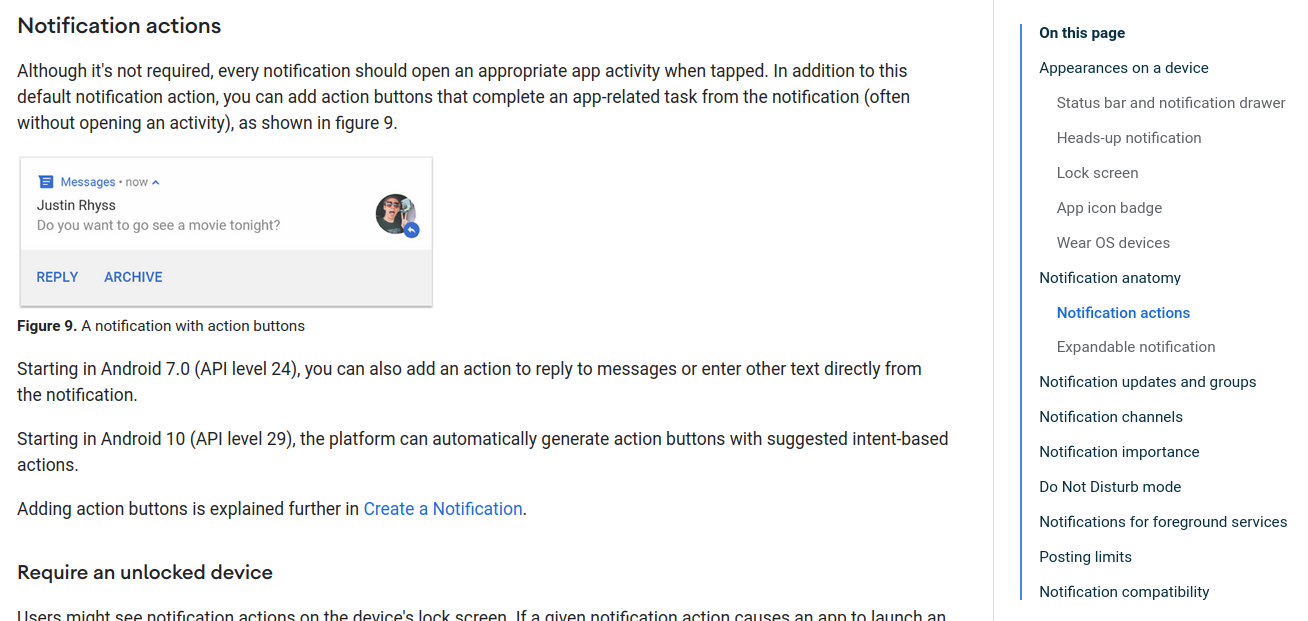
\includegraphics[width=\dimexpr\linewidth-4\fboxsep-2\fboxrule]{cp1/android-notification-documentation}
    \caption{Snapshot of the official Android Notifications API}
    \label{fig:android-notifications-api-page}
\end{figure}

\end{landscape}

